%% For double-blind review submission, w/o CCS and ACM Reference (max submission space)
\documentclass[sigplan,review,anonymous]{acmart}\settopmatter{printfolios=true,printccs=false,printacmref=false}
%% For double-blind review submission, w/ CCS and ACM Reference
%\documentclass[sigplan,review,anonymous]{acmart}\settopmatter{printfolios=true}
%% For single-blind review submission, w/o CCS and ACM Reference (max submission space)
%\documentclass[sigplan,review]{acmart}\settopmatter{printfolios=true,printccs=false,printacmref=false}
%% For single-blind review submission, w/ CCS and ACM Reference
%\documentclass[sigplan,review]{acmart}\settopmatter{printfolios=true}
%% For final camera-ready submission, w/ required CCS and ACM Reference
%\documentclass[sigplan]{acmart}\settopmatter{}

%% Conference information
%% Supplied to authors by publisher for camera-ready submission;
%% use defaults for review submission.
%\acmConference[Submitted to PLDI'18]{ACM SIGPLAN Conference on Programming Language Design and Implementation}{June 18--22, 2018}{Philadelphia, PA, USA}
\acmConference[Submitted to PLDI]{}{June 2019}{Phoenix, Arizona}
\acmYear{2019}
%\acmISBN{} % \acmISBN{978-x-xxxx-xxxx-x/YY/MM}
%\acmDOI{} % \acmDOI{10.1145/nnnnnnn.nnnnnnn}
\startPage{1}

%% Copyright information
%% Supplied to authors (based on authors' rights management selection;
%% see authors.acm.org) by publisher for camera-ready submission;
%% use 'none' for review submission.
\setcopyright{none}
%\setcopyright{acmcopyright}
%\setcopyright{acmlicensed}
%\setcopyright{rightsretained}
%\copyrightyear{2018}           %% If different from \acmYear

%% Bibliography style
\bibliographystyle{ACM-Reference-Format}
%% Citation style
%\citestyle{acmauthoryear}  %% For author/year citations
%\citestyle{acmnumeric}     %% For numeric citations
%\setcitestyle{nosort}      %% With 'acmnumeric', to disable automatic
                            %% sorting of references within a single citation;
                            %% e.g., \cite{Smith99,Carpenter05,Baker12}
                            %% rendered as [14,5,2] rather than [2,5,14].
%\setcitesyle{nocompress}   %% With 'acmnumeric', to disable automatic
                            %% compression of sequential references within a
                            %% single citation;
                            %% e.g., \cite{Baker12,Baker14,Baker16}
                            %% rendered as [2,3,4] rather than [2-4].


%%%%%%%%%%%%%%%%%%%%%%%%%%%%%%%%%%%%%%%%%%%%%%%%%%%%%%%%%%%%%%%%%%%%%%
%% Note: Authors migrating a paper from traditional SIGPLAN
%% proceedings format to PACMPL format must update the
%% '\documentclass' and topmatter commands above; see
%% 'acmart-pacmpl-template.tex'.
%%%%%%%%%%%%%%%%%%%%%%%%%%%%%%%%%%%%%%%%%%%%%%%%%%%%%%%%%%%%%%%%%%%%%%


%% Some recommended packages.
\usepackage{booktabs}   %% For formal tables:
                        %% http://ctan.org/pkg/booktabs
\usepackage{subcaption} %% For complex figures with subfigures/subcaptions
                        %% http://ctan.org/pkg/subcaption

\usepackage[utf8]{inputenc}
\usepackage[T1]{fontenc}
\usepackage[scaled=0.83]{beramono}
\usepackage{amsmath}
\usepackage{amssymb}
\usepackage{xcolor,colortbl}
\usepackage{url}
\usepackage{listings}
\usepackage{paralist}
%\usepackage[compact]{titlesec}
\usepackage[font={small}]{caption}
\usepackage{wrapfig}
\usepackage{enumitem}
\usepackage{multicol}
\usepackage{flushend}
\usepackage{bcprules}

\usepackage{tikz}
\usetikzlibrary{matrix}

% ----- listings

%\definecolor{ckeyword}{HTML}{7F0055}
\definecolor{ckeyword}{HTML}{0454cb}
\definecolor{ccomment}{HTML}{3F7F5F}
\definecolor{cstring}{HTML}{2A0099}

\lstdefinelanguage{Scala}%
{morekeywords={
  abstract,%
  case,catch,char,class,%
  def,do,else,extends,final,finally,for,%
  if,import,implicit,%
  match,module,%
  new,null,undefined,%
  fun, array,
  override,%
  package,private,protected,public,%
  for,public,return,super,%
  this,throw,trait,try,type,%
  val,var,%
  with,while,%
  object,
  let,skip,assert,then,fst,snd,root,idx,sum,prod,exists,forall,%
  yield%
  },%
  sensitive,%
  moredelim=*[il][\bfseries]{\#\#\ },
  morecomment=[l]//,%
  morecomment=[s]{/*}{*/},%
  morestring=[b]",%
  %morestring=[b]',%
  showstringspaces=false%
}[keywords,comments,strings]%

\lstset{language=Scala,%
  mathescape=true,%
%  columns=[c]fixed,%
%  basewidth={0.5em, 0.40em},%
  aboveskip=2pt,%\smallskipamount,
  belowskip=1pt,%\negsmallskipamount,
  lineskip=-1pt,
  basewidth={0.6em, 0.45em},%
%  backgroundcolor=\color{listingbg},
  basicstyle=\footnotesize\ttfamily,
  keywordstyle=\keywordstyle,
  commentstyle=\commentstyle,
  stringstyle=\stringstyle,
%  xleftmargin=0.5cm
  literate={-->}{{$\to$}}3 
           {->}{{$\mapsto$}}3 
           {=>}{{$\Rightarrow ~$}}2 
           {|-}{{$\ts$}}2 
           %{fun}{{$\lambda$}}1 
           {idx}{{$\#$}}1 
           {sum}{{$\Sigma$}}1 
           {array(}{{$\langle.\rangle$(}}3
           {σ}{{$\sigma$}}1
           {ρ}{{$\rho$}}1
           {→}{{$\to$}}1
           {λ}{{$\lambda$}}1
           {α}{{$\alpha$}}1
           %{[[}{{$[\![$}}1
           %{]]}{{$]\!]$}}1
           %{…}{{$\!...$}}1 
}

\definecolor{listingbg}{RGB}{240, 240, 240}

\newcommand{\commentstyle}[1]{\color{ccomment}\itshape{#1}}
\newcommand{\keywordstyle}[1]{\color{ckeyword}\bfseries{#1}}
%\newcommand{\keywordstyle}[1]{\color{ckeyword}{#1}}
\newcommand{\stringstyle}[1]{\color{cstring}\bfseries{#1}}

\lstnewenvironment{listing}{\lstset{language=Scala}}{}
\lstnewenvironment{listingtiny}{\lstset{language=Scala,basicstyle=\scriptsize\ttfamily}}{}

\newcommand{\code}[1]{\lstinline[language=Scala,columns=fixed,basicstyle=\ttfamily]|#1|}

% ----- packed items, so we don't waste space
\newenvironment{sitemize}{
\begin{itemize}[leftmargin=2.5ex]
  \setlength{\itemsep}{1pt}
  \setlength{\parskip}{0pt}
  \setlength{\parsep}{0pt}
}{\end{itemize}}

\newenvironment{senumerate}{
\begin{enumerate}[leftmargin=2.5ex]
  \setlength{\itemsep}{1pt}
  \setlength{\parskip}{0pt}
  \setlength{\parsep}{0pt}
}{\end{enumerate}}

\newcommand{\mypar}[1]{{\bf #1.}}

% ----- formal

%\newcommand{\judgement}[2]{{\bf #1} \hfill #2}
%\newcommand{\den}[1]{$\left\llbracket$\;#1\;$\right\rrbracket$}
\newcommand{\den}[1]{\llbracket~#1~\rrbracket}

%\newcommand{\ts}{\,\vdash\,}
\newcommand{\evalsto}{\Downarrow}

\newcommand{\mbind}{\;{\small{\texttt{>>}\hspace{-0.3pt}\raisebox{-0.15pt}{\texttt{=}}}}\;}

%\newcommand{\mbind}{{\small{\texttt{>>}\hspace{-1.7pt}\raisebox{-0.15pt}{\texttt{=}}}}}

\newcommand{\rref}[1]{\textsc{(#1)}}

% ----- comments and todo

\newcommand{\note}[1]{{\color{red}[#1]}}
\newcommand{\todo}[1]{\note{TODO: #1}}

\newcommand{\silent}[1]{}



\newcommand{\updownarrows}{\mathbin\uparrow\hspace{-.5em}\downarrow}
\newcommand{\downuparrows}{\mathbin\downarrow\hspace{-.5em}\uparrow}

\begin{document}

%% Title information
\title[Short Title]{Staged Abstract Interpreters}         %% [Short Title] is optional;
                                        %% when present, will be used in
                                        %% header instead of Full Title.
%\titlenote{with title note}             %% \titlenote is optional;
                                        %% can be repeated if necessary;
                                        %% contents suppressed with 'anonymous'
%\subtitle{Fast and Compositional Whole-Program Analysis for Free}                     %% \subtitle is optional
\subtitle{Fast and Compositional Whole-Program Analysis via Meta-Programming}                     %% \subtitle is optional
%\subtitlenote{with subtitle note}       %% \subtitlenote is optional;
                                        %% can be repeated if necessary;
                                        %% contents suppressed with 'anonymous'


%% Author information
%% Contents and number of authors suppressed with 'anonymous'.
%% Each author should be introduced by \author, followed by
%% \authornote (optional), \orcid (optional), \affiliation, and
%% \email.
%% An author may have multiple affiliations and/or emails; repeat the
%% appropriate command.
%% Many elements are not rendered, but should be provided for metadata
%% extraction tools.

%% Author with single affiliation.
\author{First1 Last1}
\authornote{with author1 note}          %% \authornote is optional;
                                        %% can be repeated if necessary
\orcid{nnnn-nnnn-nnnn-nnnn}             %% \orcid is optional
\affiliation{
  \position{Position1}
  \department{Department1}              %% \department is recommended
  \institution{Institution1}            %% \institution is required
  \streetaddress{Street1 Address1}
  \city{City1}
  \state{State1}
  \postcode{Post-Code1}
  \country{Country1}                    %% \country is recommended
}
\email{first1.last1@inst1.edu}          %% \email is recommended

%% Author with two affiliations and emails.
\author{First2 Last2}
\authornote{with author2 note}          %% \authornote is optional;
                                        %% can be repeated if necessary
\orcid{nnnn-nnnn-nnnn-nnnn}             %% \orcid is optional
\affiliation{
  \position{Position2a}
  \department{Department2a}             %% \department is recommended
  \institution{Institution2a}           %% \institution is required
  \streetaddress{Street2a Address2a}
  \city{City2a}
  \state{State2a}
  \postcode{Post-Code2a}
  \country{Country2a}                   %% \country is recommended
}
\email{first2.last2@inst2a.com}         %% \email is recommended
\affiliation{
  \position{Position2b}
  \department{Department2b}             %% \department is recommended
  \institution{Institution2b}           %% \institution is required
  \streetaddress{Street3b Address2b}
  \city{City2b}
  \state{State2b}
  \postcode{Post-Code2b}
  \country{Country2b}                   %% \country is recommended
}
\email{first2.last2@inst2b.org}         %% \email is recommended


%% Abstract
%% Note: \begin{abstract}...\end{abstract} environment must come
%% before \maketitle command
\begin{abstract}
  It is well known that a staged interpreter is a compiler: specializing the
interpreter to a given program produces an equivalent program that runs faster,
which is known as the first Futamura projection. It is even more widely known that an
abstract interpreter is a program analyzer: tweaking the interpreter to run on a
domain of abstract values produces a sound static analysis. What happens when we
combine these two ideas, and apply staging to an \emph{abstract} interpreter?

In this paper, we present a unifying framework that naturally extends the first
Futamura projection of concrete interpreters to abstract interpreters. Our
approach derives a sound staged abstract interpreter based on a
semantic-agnostic interpreter with type-level binding-time abstraction and
monadic abstraction. By using different instantiations of these abstractions,
the generic interpreter can flexibly behave in four modes: unstaged concrete
interpreter, staged concrete interpreter, unstaged abstract interpreter, or
staged abstract interpreter.

As an example of abstraction without regret, we show that staging abstract
interpreters is practical and useful to optimize static analysis while requiring
least engineering efforts and not compromising any soundness. We conduct three
case studies, including a comparison with
\citeauthor{Boucher:1996:ACN:647473.727587}'s abstract compilation,
the application on various control-flow analyses, and the use to modular
analysis. We also empirically evaluate the performance improved by staging. The
overhead of the abstraction layers is eliminated in the generated code, and the 
experiment shows an average speedup of 11x times with staging for control-flow analysis.

\iffalse
We obtain a sound static analysis, specialized for
a given program, that runs faster. More surprisingly, we show that by applying
the staged abstract interpreter to \textit{open} programs and considering the
free variables as dynamic inputs, we obtain a modular analysis that generates
sound partial analysis results which can be composed and reused later without
losing precision, even though the original abstract interpreter is a
whole-program analysis algorithm.

Based on the idea of staged abstract interpreters, we show several case studies,
including \citeauthor{Boucher:1996:ACN:647473.727587}'s abstract compilation of
0-CFA, pushdown control-flow analysis with context-sensitivity and precise
stores, and a numerical analysis on an imperative language.

We empirically evaluate the performance improvements on control-flow analysis of
benchmark programs. The results show speedups up to 2.3x with staging on a
monovariant analysis.
\fi

% It is well known that a staged interpreter is a compiler, which provides
% performance improvement by specializing the interpreter to a given program. In
% this paper, we study \textit{abstract} interpreters combined with multi-stage
% programming, i.e., the staged abstract interpreters. By staging the abstract
% interpreter with respect to a program, we obtain a specialized analysis that
% runs faster. By applying the staged abstract interpreter with \textit{open}
% programs and considering the free variables as dynamic inputs, we obtain a
% modular analysis that generates sound partial analysis results which can be
% composed and reused later without losing precision, though the original
% abstract interpreter is a whole-program analysis algorithm. Using the idea of
% staged abstract interpreters, we show several case studies, including
% \citeauthor{Boucher:1996:ACN:647473.727587}'s abstract compilation of 0-CFA,
% pushdown control-flow analysis with context/path/flow-sensitivity and
% store-widening, and a numerical analysis on an imperative language. We also
% empirically evaluate the improvement of performance on control-flow analysis
% of benchmark programs. The result shows an average speedup of Nx when staging
% to Scala for a monovariant analysis, and Mx for polyvariant analysis.

\end{abstract}


%% 2012 ACM Computing Classification System (CSS) concepts
%% Generate at 'http://dl.acm.org/ccs/ccs.cfm'.
\begin{CCSXML}
<ccs2012>
<concept>
<concept_id>10011007.10011006.10011008</concept_id>
<concept_desc>Software and its engineering~General programming languages</concept_desc>
<concept_significance>500</concept_significance>
</concept>
<concept>
<concept_id>10003456.10003457.10003521.10003525</concept_id>
<concept_desc>Social and professional topics~History of programming languages</concept_desc>
<concept_significance>300</concept_significance>
</concept>
</ccs2012>
\end{CCSXML}

\ccsdesc[500]{Software and its engineering~General programming languages}
\ccsdesc[300]{Social and professional topics~History of programming languages}
%% End of generated code


%% Keywords
%% comma separated list
% \keywords{keyword1, keyword2, keyword3}  %% \keywords are mandatory in final camera-ready submission


%% \maketitle
%% Note: \maketitle command must come after title commands, author
%% commands, abstract environment, Computing Classification System
%% environment and commands, and keywords command.
\maketitle

\section{Introduction}

Futamura projections \cite{Futamura1999, futamura1971partial} reveal the close
connection between compilers and interpreters. The first Futamura projection
specifically shows that specializing an interpreter with respect to the input
program yields an equivalent executable. Partial evaluation
\cite{DBLP:books/daglib/0072559} was the first proposed approach to realize
Futamura projections, which first identifies the binding-time of variables in
the program, i.e., they can be known whether statically or dynamically, and then
evaluates the static part, and finally generates a residual program that solely
relies on the dynamic part. However, given an arbitrary program, precisely
analyzing its binding-time is hard in general. As an alternative and pragmatic
approach to specialization and partial evaluation, multi-stage programming (MSP
for short) \cite{taha1999multi, DBLP:conf/pepm/TahaS97} requires the stage
annotations (i.e., binding-time annotations) to be explicit from the
programmers. The stage annotations can be either syntactic (as in
MetaML/MetaOCaml, through quasi-quote, escape, etc.) or type-based \todo{cite}.
These staging annotations identify which part of the inputs should be
specialized. As a classical example, we use the power function and type-based
annotations to introduce the idea of MSP:

\begin{lstlisting}
def power(b: Rep[Int], e: Int): Rep[Int] = 
  if (e == 0) 1 else b * power(b, e - 1)
\end{lstlisting}

If the programmer identifies that @b@ will be known in the future stage (as shown
on its type @Rep[Int]@ -- a representation of @Int@) and @e@ is known at the
current stage, say 5, then we can specialize the function @power@ with
respect to @e = 5@, and generate a specialized function where the overhead of
recursion is eliminated. Conceptually, the generated code looks like the following:

\begin{lstlisting}
def power5(b: Int): Int = b * b * b * b * b
\end{lstlisting}

Now to concretely illustrate the idea of Futamura projection, consider that we
have an interpreter @eval@ of some language as following:

\begin{lstlisting}
def eval(e: Expr)(arg: Input): Value = ...
\end{lstlisting}

where $e$ is the program of type @Expr@ and @arg@ is the input to program $e$,
and @eval@ produces a value.
Semantically, the interpreter satisfies $ \texttt{eval}(e)(arg) = [\![ e ]\!] arg$ for all
programs and inputs. Given a program $e_0$, by applying the first Futamura
projection, we may obtain a specialized interpreter
$\texttt{eval}_{\texttt{e0}}$ with respect to $e_0$, and by definition of the interpreter, 
$\texttt{eval}_{\texttt{e0}}(arg) = [\![ e_0 ]\!] arg $. If we generalize the
argument @arg@ to an environment (as well as a companion heap object, if for the
interest of using assignments) that contains values mapped from free variables
in $e$, the interpreter is a standard environment/store-passing interpreter,
where the specialization through MSP is also applicable.

Roughly at the same time when Futamura projections was visioned in 1970s,
\citeauthor{DBLP:conf/popl/CousotC77} proposed abstract interpretation as a
lattice-based semantic approach to construct sound static analysis, by
approximation of fix-points \cite{DBLP:conf/popl/CousotC77}. However,
constructing sound abstract interpreters was considered abstruse and complicated
for a long time.
Recent progress such as Abstracting Abstract Machines (AAM)
uncovers a systematic method to derive sound abstract interpreters from their
concrete counterparts, where the soundness can be easily established by
examining the transformation of semantics.
The AAM approach also has been been applied to different variants of
definitional interpreters and abstract machines \cite{DBLP:journals/jfp/HornM12,
  DBLP:conf/icfp/HornM10, DBLP:journals/pacmpl/DaraisLNH17}. 

\paragraph{Futamura Projection of Abstract Interpreters}

Now we have seen two orthogonal transformations of interpreters: by
specialization, we can refactor interpreters to code generators; by
approximation, we can refactor interpreters to static analyzers. As an
intellectual quest, we should naturally ask -- starting from an interpreter,
\textit{can we derive a sound abstract interpreter while it produces fast code
that does the analysis?}
Conceptually, it is similar to the concrete setting: for an
abstract interpreter $\widehat{\texttt{eval}}: \texttt{Expr} \to
\widehat{\texttt{Env}} \to \widehat{\texttt{Value}}$, which takes a program, an abstract
environment and returns abstract values, we would like to specialize it with
respect to a program $e_0$ and produce a compiled analysis
$\widehat{\texttt{eval}}_{\texttt{e0}} : \widehat{\texttt{Env}} \to
\widehat{\texttt{Value}}$, such that $
\widehat{\texttt{eval}}_{\texttt{e0}}(\widehat{\rho}) =
\widehat{\texttt{eval}}(e_0)(\widehat{\rho})$, but the compiled one leaves the
abstract environment $\widehat{\rho}$ as remaining input.

\begin{figure}[h]
  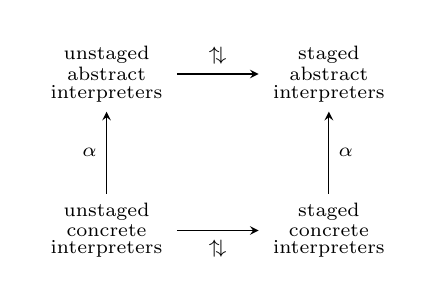
\begin{tikzpicture}
  \matrix (m) [matrix of math nodes,row sep=3em,column sep=3em,minimum width=2em]
  {
    \begin{smallmatrix} \text{unstaged} \\ \text{abstract} \\ \text{interpreters} \end{smallmatrix} & \begin{smallmatrix} \text{staged} \\ \text{abstract} \\ \text{interpreters} \end{smallmatrix} \\
      \begin{smallmatrix} \text{unstaged} \\ \text{concrete} \\ \text{interpreters} \end{smallmatrix} & \begin{smallmatrix} \text{staged} \\ \text{concrete} \\ \text{interpreters} \end{smallmatrix} \\ };
  \path[-stealth]
    (m-1-1) edge node [above, font=\scriptsize] {$\updownarrows$} (m-1-2)
    (m-2-1) edge node [left, font=\scriptsize] {$\alpha$} (m-1-1)
    (m-2-1) edge node [below, font=\scriptsize] {$\updownarrows$} (m-2-2)
    (m-2-2) edge node [right, font=\scriptsize] {$\alpha$} (m-1-2);
  \end{tikzpicture}
  \caption{The confluence of specialization and approximation.}
  \label{confluence}
\end{figure}

In this paper, we study the confluence of two old ideas --- Futamura projection
and abstract interpretation, but from the perspective of their recent
realizations --- multi-stage programming and definitional abstract interpreters.
To be specific, we present the application of the first Futamura projection on
definitional abstract interpreters, which intersects as staged abstract
interpreters. By borrowing the ideas from monadic interpreters
\cite{Steele:1994:BIC:174675.178068, DBLP:conf/popl/LiangHJ95,
DBLP:journals/pacmpl/DaraisLNH17, Sergey:2013:MAI:2491956.2491979} and embedded
domain-specific languages \cite{DBLP:conf/snapl/RompfBLSJAOSKDK15,
DBLP:journals/jfp/CaretteKS09, DBLP:conf/icfp/GibbonsW14,
Hofer:2008:PED:1449913.1449935}, we develop an approach to fulfill four
different semantics (Figure~\ref{confluence}) in a unified framework. The four
semantics share one same generic interpreter interface. Later, by instantiating
the interpreter differently, it can behave as a concrete interpreter, an
abstracter interpreter, or their code-generator versions, respectively. The key
idea that enables this flexibility is to use abstract type members abstract over
concrete/abstract components (e.g., concrete values or abstract values), as well
as the binding-time of them (e.g., static or dynamic). By staging, the overhead
caused by the monadic layers is eliminated in the generated code.

\paragraph{Performance via Specialization}

Besides the intellectual merit shown in the confluence diagram, this paper
contributes to a practical problem in static analysis: \textit{can we speed up a
static analyzer without any intrusive changes and soundness compromises?} Static
analysis is known as a trade-off game between \textit{precision} and
\textit{efficiency}, we argue that applying meta-programming (multi-stage
programming, in particular) with abstract interpreters is an effective approach
to improve the latter one while the former one is untouched. Specialization
removes the overhead of abstractions introduced by high-level programming (e.g.,
monads), but not loses any advantages of this programming style (e.g.,
extensibility), nor changes the meaning of the program -- in this case, the
abstract semantics that does the analysis. Indeed, specializing analysis
with respect to a program by partial evaluation \cite{damian1999partial,
amtoft1999partial, Boucher:1996:ACN:647473.727587, ashley:practical} is not a
new idea, despite the fact that most of the previous work are ad-hoc on a
particular analysis or requiring significant changes to the analysis. For
example, abstract compilation \cite{Boucher:1996:ACN:647473.727587} requires the
whole analyzer to be rewritten as closure generation from. In this paper, we
show a systematic approach to meta-programming that achieves the performance
goal with less intrusive changes; in fact, a case study (Section~\ref{cs_ac})
comparing with abstract compilation shows, by utilizing type-based stage
annotations, the analyzer program does not need any changes.

\paragraph{Modularity via Meta-Programming}

Our second contribution is to enable modular analysis based on a whole-program
analyzer by meta-programming. Modern software are shipped with large libraries
\cite{toman_et_al:LIPIcs:2017:7121}, and analyzing programs with large libraries
is usually expensive or unnecessarily repeated for whole-program analyzing
algorithms. For example, it has been shown that analyzing a simple ``Hello
World'' program in Java depends on additional 3,000 classes in the library
\cite{DBLP:conf/oopsla/KulkarniMZN16}. A natural idea is to analyze libraries
and generate summaries, later we can plugin the necessary information into the
summaries and finish the analysis; therefore such summaries should be modular
and reusable. Meta-programming gives us a chance to readily tweak a
whole-program analyzing algorithm into an analyzer that works modularly and
produces summaries. Still, the idea is to specialize the abstract interpreter
that was used for whole-program analysis, but on a subset of the program, for
examples, several generic functions for list manipulation. Such specialization
works on lambda expressions and generates code, which is partial analysis
results and can be completed by running with the necessary arguments (for
example, an environment that closes the lambda term) at next stages. Multiple
partial analysis results also can be reused later and composed together as they
are just normal programs at the next stage. Through staging, we mechanically
obtain a modular analysis, even though the original algorithm is formulated as a
whole-program analysis.

\iffalse
Likewise, specializing static analyses by partial evaluation emerged in late 90s
, and indeed it is able to effectively remove the interpretive
overhead of repeatedly traversing the abstract syntax tree. However, these
previous works focused mostly on one particular analysis, or required to
completely rewrite the analyzer. Hence, it is worth to investigate the idea from
a modern perspective based on generative programming, especially for a general
abstract interpreter that models direct-style $\lambda$-calculus, imperative
features such as mutation, and different abstract domains. One technical
challenge is the binding-time engineering when non-determinism, fixed-point
iterations, different abstract domains and staging are introduced at the same
time. In this paper, we present an end-to-end design and implementation of
staging an abstract interpreter; that means not only the interpreter that
traverses the abstract syntax tree, but also the data structure of abstract
domains, abstract environment and heap, and the fixed-point iteration are
staged.

\todo{rewrite this paragraph}
On the other hand, the abstract interpreter, as a semantic artifact, should be
written in a style that is easy for people to communicate the formulation and
abstraction, but also can be implemented efficiently. As the slogan of
multi-stage programming said, "abstraction without regret", we draw connection
between high-level description and efficient implementation of abstract
interpreters, just like the connection between concrete interpreters and
compilers drawn by Futamura projection. Particularly, we show an easy but
systematic way of adding stage annotations to the abstract interpreter without
changing the code of the interpreter skeleton, which is shared between four concrete
or abstract, unstaged or staged interpreters. We use the LMS framework for staging,
which allows us only use types to annotate the binding-time. Therefore, the
proposed approach bridges the gap between designing sound static analysis and
implementing efficient program analyzer.

%Of course, all interpreters are metalinguistic abstractions, but some
%interpreters are more "abstract" than others \todo{maybe rephrase}.
%Particularly, we also would like a systematic approach to optimize program
%analyzers and meanwhile minimally modifying the analyzer programs.

When staging a concrete interpreter, the programmers need to distinguish static
and dynamic values --- the given program to be executed by the interpreter is
classified as static because it is known at compile-time, and the inputs to that
program are dynamic. However, when staging an abstract interpreter, this
distinction does not exist anymore. Because the abstract interpreter
instantiates all the inputs as some form of abstract values, which are usually
top elements in their abstract domains and are also statically known. Then what
is the point of staging if there is no such distinction? A surprising by-product
of thinking about this question is to realize that we can apply the staged
abstract interpreter on \textit{open} programs, and the free variables
representing other parts of the program (e.g., libraries) are dynamic inputs,
therefore we obtain a modular analysis through staging, mechanically.
\note{TR: I don't understand this. The program structure is static, the abstract values
are still dynamic, no? They change in every iteration of the fixpoint algorithm}
\note{TR: why is it a big deal. On Closed programs we obtain a constant factor,
but modular analysis has different asymptotics}

When targeting higher-order programs, either staged concrete interpreters or
staged abstract interpreters are able to compile a closure, i.e., specialize the
call of interpreter with respect to the body expression of the lambda term
without knowing the actual argument value. By generalizing this observation, we
can actually specialize the abstract interpreter with any open programs, which
unexpectedly leads to a modular analysis and improves scalability. An open
program contains free variables, which represent other parts of the program and
will be left as dynamic values. For instance, one challenge in static analysis
of modern software is that the programs are usually shipped with large library
code \cite{toman_et_al:LIPIcs:2017:7121}, for example, it has been shown that
analyzing a simple "Hello World" program in Java depends on additional 3,000
classes in the library \cite{DBLP:conf/oopsla/KulkarniMZN16}. A precise
whole-program analysis formulated as abstract interpreters can be very expensive
due to the scale of the program and the inherent complexity of the algorithm.
However, analyzing these libraries is sometimes unnecessarily repeated. When
applying the staged abstract interpreter on such open programs, we leave the
unknown arguments and calling contexts as dynamic values and generate partial
analyzing result which is represented as a residual program. The partial
analyzing result can be reused and composed with the analyzing result of
application code when available later. Therefore we mechanically obtain a
modular analysis through staging, even though the original algorithm is
formulated as a whole-program analysis.

It has been observed that partially applying context-sensitivity on selected
portion of the program could improve the precision and efficiency
\cite{zipper2018, Kastrinis:2013:HCP:2491956.2462191}. We show that staging
abstract interpreters as an approach to effectively implement hybird
context-sensitivity\todo{}.
\fi

%\note{Expression problem \cite{DBLP:conf/icfp/GibbonsW14, DBLP:conf/ecoop/KrishnamurthiFF98, expproblem},}

\paragraph{Contributions and Outline}

\begin{itemize}
  \item We progressively present a unifying construction that naturally extends
    the first Futamura projection to abstract interpreters. Starting from a generic
    interface of the interpreter for a small functional language
    (Section~\ref{generic_if}), we first show the instantiation of concrete
    interpretation (Section~\ref{unstaged_conc}). Then we lift it to the staged
    version by replacing the binding-time type (Section~\ref{stagedinterp}); and to
    the abstract interpreter by applying abstraction to the environment, store, and
    values (Section~\ref{unstaged_abs}). Finally, we show the combination of the two
    transformations, dubbed \textit{staged abstract interpreters}, can be easily
    derived (Section~\ref{sai}).

  \item We demonstrate that if we apply the abstract interpreter on components
    of the program separately, it not only improves the \textit{efficiency} but
    also the \textit{scalability} (Section~\ref{sai} \todo{}), which are two
    major issues in static analysis.

  \item We conduct two case studies to show the applicability and usefulness
    of applying meta-programming to static analysis (Section~\ref{cases_study}).
    (1) We first revisit the Abstract Compilation (AC)
    \cite{Boucher:1996:ACN:647473.727587} technique (Section~\ref{cs_ac}).
    Our approach and AC are able to achieve the same goal, however, as we show,
    one of the advantage of staging through types is it does not require
    whole-analyzer refactoring.
    (2) We extend the staged abstract interpreter to two variants of
    control-flow analysis: context-sensitive pushdown control-flow analysis and
    \todo{precise-store?} (Section~\ref{sai}).
    
  \item Based on the instantiation of control-flow analysis, we empirically
    evaluate the performance improvement by staging and specialization
    (Section~\ref{evaluation}). We compare the both context-insensitive and
    \note{context-sensitive} analysis.
    
\end{itemize}

\newcommand{\TLang}{$L_\lambda$}

\section{Preliminaries}

In this section, we first describe the abstract syntax of the language we will
analyze, then present the generic interface shared between the four different
interpreters. We choose to use Scala to demonstrate the idea, but the idea of
using monads and multi-stages also can be easily constructed in other functional
languages, such as MetaOCaml.
We first instantiate the interpreter to the concrete one; then we
proceed in two directions: by staging it we obtain a staged concrete interpreter
(Section~\ref{stagedinterp}), by abstracting it we obtain an unstaged abstract
interpreter (Section~\ref{unstaged_abs});

\subsection{Abstract Syntax} \label{bg_lang}

We consider a tiny higher-order functional language \TLang, which is based on
direct-style $\lambda$-calculus with numbers, arithmetics, recursions and
conditionals. In Section~\ref{cases_imp}, we will add more imperative features
to the language. Since we are mostly interested in analyzing the dynamic
behavior of the program, we disguised any static semantics and type system. We
also assume that input programs are well-typed and variables are distinct. The
abstract syntax is as follows:

\begin{lstlisting}
abstract class Expr
case class Lit(i: Int)                         // numbers
case class Var(x: String)                      // variables
case class Lam(x: String, e: Expr)             // lambda abstractions
case class App(e1: Expr, e2: Expr)             // applications
case class AOp(op: String, e1: Expr, e2: Expr) // primitive operations
case class Rec(x: String, rhs: Expr, e: Expr)  // recursive bindings
case class If0(e1: Expr, e2: Expr, e3: Expr)   // conditionals
\end{lstlisting}

We give the concrete semantics of \TLang by showing a big-step definitional
interpreter. The interpreter is a recursive function that takes the program AST,
environment and store, and returns the evaluated value and the accompanied
store. The environment is a mapping from identifiers to addresses, and the store
is a mapping from addresses to values. We use the store to model recursion and
mutation in concrete semantics; it is also useful for polyvariant analysis. This
environment-and-store-passing style big-step interpreter is standard and can
also be obtained by refunctionalizing \cite{DBLP:conf/ppdp/AgerBDM03,
Wei:2018:RAA:3243631.3236800} a small-step CESK machine
\cite{DBLP:conf/popl/FelleisenF87}.

\subsection{Generic Interface} \label{generic_if}

Before showing the actual implementation of the concrete semantics, let us first
consider a generic interface for the interpreters, which is semantics-agnostic
and can be "interpreted" by either concrete or abstract, unstaged or staged
semantics of our choice. The trait \texttt{Semantics} first declares several
abstract type members, such as \texttt{Addr}, \texttt{Value}, \texttt{Env},
\texttt{Store} and returned type \texttt{Ans}. It also declares initial values
for environments and stores, and few abstract methods that manipulate
environments and stores such as @put@ and @get@.

\begin{lstlisting}
trait Semantics {
  type R[+_]
  type Ident = String;  type Addr;  type Value;  type Env
  type Store;  type Ans = (R[Value], R[Store])
  def get($\rho$: R[Env], x: Ident): R[Addr]
  def put($\rho$: R[Env], x: Ident, a: R[Addr]): R[Env]
  def get($\sigma$: R[Store], a: R[Addr]): R[Value]
  def put($\sigma$: R[Store], a: R[Addr], v: R[Value]): R[Store]
  def alloc($\sigma$: R[Store], x: Ident): R[Addr]
  val $\rho$0: R[Env]; val $\sigma$0: R[Store]
  def close(ev: EvalFun)($\lambda$: Lam, $\rho$: R[Env]): R[Value]
  def num(i: Lit): R[Value]
  def apply_closure(ev: EvalFun)
    (f: R[Value], arg: R[Value], $\sigma$: R[Store]): Ans
  def branch0(cnd: R[Value], thn: => Ans, els: => Ans): Ans
  def prim_eval(op: Symbol, v1: R[Value], v2: R[Value]): R[Value]
}  // to be continued
\end{lstlisting}

The actual semantics and operations of the interpreter are left to be
implemented later, these include operations such as lifting literal terms to
values (\texttt{close}, \texttt{num}), applying a closure
(\texttt{apply\_closure}), branching (\texttt{branch0}), and arithmetics
(\texttt{prim\_eval}). We can choose to implement them in a way that is concrete
or abstract, unstaged or staged. But, just based on these abstract operations,
an expressive generic interpreter can be defined:

\begin{lstlisting}
trait Semantics {  // continued
  type EvalFun = (Expr, R[Env], R[Store]) => Ans
  def eval(ev: EvalFun)(e: Expr, $\rho$: R[Env], $\sigma$: R[Store]): Ans = 
    e match {
      case Lit(i) => (num(Lit(i)), $\sigma$)
      case Var(x) => (get($\sigma$, get($\rho$, x)), $\sigma$)
      case Lam(x, e) => (close(ev)(Lam(x, e), $\rho$), $\sigma$)
      case App(e1, e2) =>
        val (e1v, e1$\sigma$) = ev(e1, $\rho$, $\sigma$)
        val (e2v, e2$\sigma$) = ev(e2, $\rho$, e1$\sigma$)
        apply_closure(ev)(e1v, e2v, e2$\sigma$)
      case Rec(x, f, body) =>
        val $\alpha$ = alloc($\sigma$, x)
        val $\rho$_* = put($\rho$, x, $\alpha$)
        val (fv, f$\sigma$) = ev(f, $\rho$_*, $\sigma$)
        val $\sigma$_* = put(f$\sigma$, $\alpha$, fv)
        ev(body, $\rho$_*, $\sigma$_*)
      case If0(cnd, thn, els) =>
        val (cndv, cnd$\sigma$) = ev(cnd, $\rho$, $\sigma$)
        branch0(cndv, ev(thn, $\rho$, cnd$\sigma$), ev(els, $\rho$, cnd$\sigma$))
      case AOp(op, e1, e2) =>
        val (e1v, e1$\sigma$) = ev(e1, $\rho$, $\sigma$)
        val (e2v, e2$\sigma$) = ev(e2, $\rho$, e1$\sigma$)
        (prim_eval(op, e1v, e2v), e2$\sigma$)
    }
  def fix(ev: EvalFun => EvalFun): EvalFun = 
    (e, $\rho$, $\sigma$) => ev(fix(ev))(e, $\rho$, $\sigma$)
  def eval_top(e: Expr): Ans = eval_top(e, $\rho$0, $\sigma$0)
  def eval_top(e: Expr, $\rho$: R[Env], $\sigma$: R[Store]): Ans = 
    fix(eval)(e, $\rho$, $\sigma$)
}
\end{lstlisting}

The implementation of the skeleton interpreter traverses the abstract syntax
tree and should be straightforward to understand. It is worth noting that the
interpreter is written in open-recursive style -- it can not refer to itself
directly, instead, \texttt{eval} takes an additional parameter \texttt{ev}
referring to itself; this allows us to instrument the interpreter from the
outside. Accordingly, the function \texttt{close} for lifting lambda term to
closure values is also written in this style. We define a default implementation
\texttt{fix} to close the recursion by recursively using the result of
\texttt{fix(ev)} for \texttt{ev}. Finally, the top-level evaluation function
\texttt{eval\_top} is defined.

\paragraph{Stage Polymorphism}

Readers may notice that an abstract higher-kinded type \texttt{R[+T]} is defined
in the trait, i.e. a type-level function which will be used to specify the
binding-time, i.e., staged or not; the annotation \texttt{+} indicates that the
type parameter \texttt{T} is covariant. The LMS framework we use here allows us
to specify binding-times purely based on types. All occurrences of type
\texttt{Env}, \texttt{Store}, etc. are wrapped with \texttt{R} essentially
because they may potentially be dynamic when staging is introduced. Obviously,
the unstaged higher-kinded type then can be simply instantiated as an identity
type function: \texttt{type R[+T] = T}. In Section~\ref{stagedinterp},
\texttt{R} will be instantiated as a staging annotation.

\todo{Finally tagless, poly embedding}

\subsection{Concrete Instantiation} \label{unstaged_conc}

Now we can instantiate a concrete interpreter. We first concretize the abstract
types as follows. Since the interpreter is concrete, for the purpose that
properly models the heap, the type \texttt{Int} is used for address space
\texttt{Addr}. The environment and store are just ordinary \texttt{Map}s in
Scala. A value can be either a tagged number \texttt{NumV} or a closure
\texttt{CloV} that contains a lambda term and an environment.

\begin{lstlisting}
trait Concrete extends Semantics {
  type Addr = Int;   sealed trait Value
  case class CloV($\lambda$: Lam, $\rho$: Env) extends Value
  case class NumV(i: Int) extends Value
  type Env = Map[Ident, Addr];  type Store = Map[Addr, Value]
}
\end{lstlisting}

We proceed to implement the components that define the semantics. As mentioned
before, type \texttt{R} is concretized as an identity type function, thus all
types are just ordinary types.

\begin{lstlisting}
object ConcInterp extends Concrete {
  type R[+T] = T
  val $\rho$0 = Map[Ident,Addr]();  val $\sigma$0 = Map[Addr,Value]()
  def get($\rho$: Env, x: Ident): Addr = $\rho$(x)
  def put($\rho$: Env, x: Ident, a: Addr): Env = $\rho$ + (x -> a)
  def get($\sigma$: Store, a: Addr): Value = $\sigma$(a)
  def put($\sigma$: Store, a: Addr, v: Value): Store = $\sigma$ + (a -> v)
  def alloc($\sigma$: Store, x: Ident): Addr = $\sigma$.size + 1
  def close(ev: EvalFun)($\lambda$: Lam, $\rho$: Env): Value = CloV($\lambda$, $\rho$)
  def num(i: Lit): Value = NumV(i.i)
  def apply_closure(ev: EvalFun)
    (f: Value, arg: Value, $\sigma$: Store): Ans = f match {
      case CloV(Lam(x, e), $\rho$) =>
        val $\alpha$ = alloc($\sigma$, x); val $\rho$_* = put($\rho$, x, $\alpha$)
        val $\sigma$_* = put($\sigma$, $\alpha$, arg); ev(e, $\rho$_*, $\sigma$_*)
    }
  def branch0(cnd: Value, thn: => Ans, els: => Ans): Ans = 
    cnd match { case NumV(i) => if (i == 0) thn else els }
  def prim_eval(op: Symbol, v1: Value, v2: Value): Value = 
    op match {
      case '+ => v1.asInstanceOf[NumV].i + v2.asInstanceOf[NumV].i
      ...
    }
}
\end{lstlisting}

Finally, \texttt{get} and \texttt{put} directly manipulate the map of
environment and store. An allocation function is used when we need to update the
store: in the concrete case, \texttt{alloc} always returns a fresh address of
the store. \texttt{close} and \texttt{num} lift syntactic literals to values.
\texttt{apply\_closure} takes the function value, argument value and the latest
store, then extends the environment and store after allocating a fresh address,
and continue evaluating the body \texttt{e} of the lambda term.

\section{From Interpreters to Staged Interpreters} \label{stagedinterp}

\subsection{Multi-Stage Programming in LMS}

Lightweight modular staging (LMS) \cite{DBLP:conf/gpce/RompfO10} is a
multi-stage programming framework implemented as a Scala library that enables
dynamic code generation in a type-safe manner. Different from the syntactic
approach in MetaOCaml \cite{DBLP:conf/flops/Kiselyov14,
DBLP:conf/gpce/CalcagnoTHL03} that uses quotations, LMS distinguishes
binding-time solely based on types. LMS provides a type constructor @Rep[T]@
where @T@ can be an arbitrary type, indicating an expression will be known at
next stage. All operations acting on a @Rep[T]@ expression will be residualized
in the generated code. However, we need to provide intermediate representation
and code generation support for type @T@ to LMS. Fortunately, the LMS framework
already provides such support for primitive types and commonly used data
structure such as arrays and maps; implementing such support for custom class is
also straightforward. Let's go back and see how LMS can be used to specialize
the power function we mentioned in Section 1.

\begin{lstlisting}
new DslDriver[Int, Int] {
  def power(b: Rep[Int], x: Int): Rep[Int] =
    if (x == 0) 1 else b * power(b, x-1)
  def snippet(x: Rep[Int]): Rep[Int] = power(x, 5)
}
\end{lstlisting}

In the code shown above, \texttt{power} takes two arguments where \texttt{b} is
declared as \texttt{Rep[Int]} type meaning that \texttt{b} is a representation
of \texttt{Int} but whose value will be available at the next stage. Meanwhile,
the result of the @power@ function will be available at the next stage as well,
thus the return value of \texttt{power} is also of type \texttt{Rep[Int]}. Then
we specialize @power@ in function @snippet@ by providing @x@ to @5@. The
generated code for \texttt{power5} is a function that takes only one argument
which corresponds to @b@, and the body of this function multiplies @b@ five
times.

\subsection{Staged Concrete Semantics}

In the staging part, we share the same concrete type instantiation, i.e., trait
\texttt{Concrete}, but we reimplement the staged version for the concrete
operations in trait @RepConcInterpOps@. Meanwhile, it is also extended from
@LMSOps@ which provides necessary support for the staged version of primitive
types and data structures. To stage the interpreter, we first identify the
syntactic input that is known statically, and the interpreter returns a pair of
values and store, which both becomes dynamic values. Thus the staged stores
propagate the binding-time to environments, because they share the same address
component.

\begin{lstlisting}
trait RepConcInterpOps extends Concrete with LMSOps {
  type R[+T] = Rep[T]
  val $\rho$0: Rep[Env] = Map[Ident,Addr]()
  val $\sigma$0: Rep[Store] = Map[Addr,Value]()
  def get($\rho$: Rep[Env], x: Ident): Rep[Addr] = $\rho$(x)
  def put($\rho$: Rep[Env], x: Ident, a: Rep[Addr]): Rep[Env] = 
    $\rho$ + (unit(x) -> a)
  def get($\sigma$: Rep[Store], a: Rep[Addr]): Rep[Value] = $\sigma$(a)
  def put($\sigma$: Rep[Store], a: Rep[Addr], v: Rep[Value]): Rep[Store] = 
    $\sigma$ + (a -> v)
  def alloc($\sigma$: Rep[Store], x: Ident): Rep[Addr] = $\sigma$.size + 1
  def num(i: Lit): Rep[Value] = lift(NumV(i))
  def branch0(cnd: Rep[Value], thn: => Ans, els: => Ans): Ans = {
    //FIXME: the cast is ugly, patten match?
    val i = cnd.asInstanceOf[Rep[NumV]].i
    if (i == 0) thn else els
  }
  def prim_eval(op: Symbol, 
    v1: Rep[Value], v2: Rep[Value]): Rep[Value] = op match {
      case '+ => v1.asInstanceOf[Rep[NumV]].i + 
                 v2.asInstanceOf[Rep[NumV]].i
      ...
    }
  ...
}
\end{lstlisting}

The first notable change is that the abstract type member @R@ is assigned to be
@Rep@, and accordingly the affected types such as @Env@ and @Store@ become
@Rep[Env]@ and @Rep[Store]@. For @num@, we use the @lift@ function which is a
built-in in LMS that lifts a current-stage value to next stage. The interesting
point is how we handle closures and function applications when staging is
involved. In the unstaged version, function @close@ is used to lift a literal
lambda term to a closure, which is a pair of the syntactic lambda term and the
enclosing environment. However, what we desire is a \textit{compiled} closure,
instead of a lifted @CloV@ value like what we did for @NumV@ --- in other words,
the syntactic term of the lambda expression should be eliminated and specialized
away. The specialization of the interpreter with respect to the body of the
lambda term proceeds under the assumptions that the argument and latest store
will be provided later.
%\note{to denotational style?, back to HO?}
We will see this is an important observation that enables us to specialize an
abstract interpreter in a modular way. At the end of function @close@, we create
a @CompiledClo@ object that contains a staged function, which all will be
emitted in the generated code.

\begin{lstlisting}
def close(ev: EvalFun)($\lambda$: Lam, $\rho$: Rep[Env]): Rep[Value] = {
  val Lam(x, e) = $\lambda$
  val f: Rep[(Value,Store)]=>Rep[(Value,Store)] = { 
    case (arg: Rep[Value],$\sigma$: Rep[Store]) =>
      val $\alpha$ = alloc($\sigma$, x)
      ev(e, put($\rho$, x, $\alpha$), put($\sigma$, $\alpha$, arg)) 
  }
  CompiledClo(fun(f))
}
\end{lstlisting}

Next, @apply_closure@ takes three arguments: the function value, argument value
and the latest store, which are all of @Rep@ type. This means basically there
is nothing we can do at the current stage --- so we create a new node
@ApplyClosure@ that contains these arguments in the intermediate representation
graph, and in the code generation phase we can emit the code that performs the
application. The additional @reflectEffect@ is a function in LMS that handles
side effects.

\begin{lstlisting}
case class ApplyClosure(f: Rep[Value], 
  arg: Rep[Value], $\sigma$: Rep[Store]) extends Def[(Value, Store)]
def apply_closure(ev: EvalFun)
  (f: Rep[Value], arg: Rep[Value], $\sigma$: Rep[Store]): Ans = {
    reflectEffect(ApplyClosure(f, arg, $\sigma$))
  }
\end{lstlisting}

\paragraph{Code Generation}

When generating code for the next stage, values like @CompiledClo@ and @NumV@
are kept as they are because they are intended exist in the next stage; however,
we need to treat @ApplyClosure@ a little differently.

\begin{lstlisting}
  case ApplyClosure(f, arg, $\sigma$) => 
    emitValDef(sym, quote(f) + 
                    ".asInstanceOf[CompiledClo].f(" + 
                    quote(arg) + "," + 
                    quote($\sigma$) + ")")
\end{lstlisting}

Concretely, as shown in the code above, when emitting code for @ApplyClosure@,
we just emit a function application where the function value is extracted from
the @CompiledClo@ object (we assume the input program is well-typed so that we
can safely cast it to @CompiledClo@). Argument and a store are the remaining rest
fields in @ApplyClosure@.

\section{From Interpreters to Abstract Interpreters} \label{unstaged_abs}

Based on the generic interface we presented in Section~\ref{bg_lang}, 
now we describe the instantiation of an abstract interpreter.
To keep the simplicity, we intend to use simply abstract domains, and just establish a 
context-/path-/flow-insensitive, store-widened analysis in this section --- indeed, it is coarse
but simple enough to setup a foundation for the staged abstract interpreter we will present later.
However, in Section~\ref{cfa}, we will see how to regain context-/path-/flow-sensitivity 
for pushdown control-flow analysis; in Section~\ref{cases_imp}, we will see how to instantiate 
an interval abstract domain for numerical analysis.

\todo{maybe put to related work} other big-step abstract interpreter, 
big-step abstract interpreter using delimited control operators \cite{Wei:2018:RAA:3243631.3236800},
monadic big-step abstract interpreter \cite{DBLP:journals/pacmpl/DaraisLNH17},
arrow-based abstract interpreter \cite{Keidel:2018:CSP:3243631.3236767}.

\paragraph{Abstract Instantiation.}
Our instantiation roughly follows the Abstracting Abstract Machines methodology 
\cite{DBLP:conf/icfp/HornM10, DBLP:journals/jfp/HornM12} that transforms the concrete semantics 
to abstract semantics. The store now maps addresses to sets of abstract values, meaning that an address points
to all possible values may occur at runtime, where the abstract value is either a closure or 
a single abstract number \texttt{NumV}, which stands for the top. The address space is also
constrained to be finite, in the monovariant setting, we simply use variable names for it.

\begin{lstlisting}
trait Abstract extends Semantics {
  case class Addr(x: Ident);  sealed trait AbsValue
  case class CloV($\lambda$: Lam, $\rho$: Env) extends AbsValue
  case class NumV() extends AbsValue
  type Value = Set[AbsValue]
  type Env = Map[Ident, Addr];  type Store = Map[Addr, Value]
}
\end{lstlisting}

\subsection{Stage Polymorphic Lattices} \label{stagedpoly_lat}
To effectively reuse the code between unstaged and staged part, we also make the lattice structure to
be stage polymorphic. A lattice type class parameterizes over an element type \texttt{E} and defines
five operations for \texttt{R[E]}, such as meet, join, and ordering relation; again, \texttt{R} 
is the higher-kinded type indicating the binding-time.
\begin{lstlisting}
trait Lattice[E, R[+_]] {
  val bot: R[E];  val top: R[E]
  def $\sqsubseteq$(l1: R[E], l2: R[E]): R[Boolean]
  def $\sqcup$(l1: R[E], l2: R[E]): R[E]
  def $\sqcap$(l1: R[E], l2: R[E]): R[E]
}
\end{lstlisting}

For example, here we use powerset as the abstract domain, and the unstaged lattice 
of powerset can be easily implemented as follows:

\begin{lstlisting}
implicit def SetLattice[T]: Lattice[Set[T], NoRep] = 
  new Lattice[Set[T], NoRep] {
    lazy val bot: Set[T] = Set[T]()
    lazy val top: Set[T] = throw new NotImplementedError()
    def $\sqsubseteq$(l1: Set[T], l2: Set[T]): Boolean = l1 subsetOf l2
    def $\sqcup$(l1: Set[T], l2: Set[T]): Set[T] = l1 union l2
    def $\sqcap$(l1: Set[T], l2: Set[T]): Set[T] = l1 intersect l2
  }
\end{lstlisting}

The ordering relation is to ask whether one set is a subset of the other, 
join is to union the two set, and meet is to intersect the two sets.
Accordingly, other structures used in the rest of the paper such as tuples 
(products) and maps can be lifted to lattices element-wise or point-wise.
The code for them are elided.

\subsection{Abstract Semantics}
The operations @get@ and @put@ on abstract stores are slightly changed according to
the abstract semantics: @get@ uses the bottom element in the @Value@ lattice if the 
queried address not exists; @put@ performs the update by joining with the existing values.
@alloc@ simply invokes the @Addr@ constructor.
\texttt{close} and \texttt{num} lift syntactic literals to our abstract domain, i.e., 
a singleton set that contains only one \texttt{CloV} or \texttt{NumV} object.

\todo{conditional, use different store?}
\begin{lstlisting}
object AbsInterp extends Abstract {
  type R[+T] = T
  val $\rho$0 = Map[Ident, Addr]();  val $\sigma$0 = Map[Addr, Value]()
  def get($\rho$: Env, x: Ident): Addr = $\rho$(x)
  def put($\rho$: Env, x: Ident, a: Addr): Env = $\rho$ + (x -> a)
  def get($\sigma$: Store, a: Addr): Value = 
    $\sigma$.getOrElse(a, Lattice[Value].bot)
  def put($\sigma$: Store, a: Addr, v: Value): Store =
    $\sigma$ + (a -> (v $\sqcup$ get($\sigma$, a)))
  def alloc($\sigma$: Store, x: Ident): Addr = Addr(x)
  def close(ev: EvalFun)($\lambda$: Lam, $\rho$: Env): Value = Set(CloV($\lambda$, $\rho$))
  def num(i: Lit): Value = Set(NumV())
  def apply_closure(ev: EvalFun)
    (fs: Value, arg: Value, $\sigma$: Store): Ans = { var $\sigma$_* = $\sigma$
      val vs = for (CloV(Lam(x, e), $\rho$) <- fs) yield {
        val $\alpha$ = alloc($\sigma$_*, x)
        val (v, v$\sigma$) = ev(e, put($\rho$, x, $\alpha$), put($\sigma$_*, $\alpha$, arg))
        $\sigma$_* = v$\sigma$; v
      }
    (vs.reduce(Lattice[Value].$\sqcup$), $\sigma$_*)
  }
  def branch0(cnd: Value, thn: =>Ans, els: =>Ans): Ans = 
    thn $\sqcup$ els
  def prim_eval(op: Symbol, v1: Value, v2: Value): Value = 
    Set(NumV())
} // to be continued
\end{lstlisting}

For branching, @branch0@ simply joins the answer from two branches. For arithmetics, @prim_eval@ simply 
returns the top abstract number element.
It is worth to note that @apply_closure@ is where we handle the non-determinism of applications.
The non-determinism happens because of the abstract store maps addresses to sets of abstract values;
when dereferencing an address from the store, we need to explore all possible values to achieve a sound 
analysis. In the case of @apply_closure@, the first argument @fs@ may contains multiple target closures,
so we have a @for@ comprehension over all closures, apply them respectively and form a set result values @vs@;
meanwhile, every time when we evaluate into the body expression @e@ we use the latest store $\sigma$@_*@
which is updated iteratively. Thus it is a store-widened analysis.


\subsection{Fixpoint Iteration}
We described the abstract semantics modularly in the last section, however, the abstract 
interpreter may not terminate for some input program. In this section, we use a memoization
technique to ensure its termination. This technique is also widely used in the name of co-inductive caching algorithm
\cite{DBLP:journals/pacmpl/DaraisLNH17, Wei:2018:RAA:3243631.3236800} or truncated depth-first evaluation 
\cite{Rosendahl:AbsIntPL}.

The idea is to set up two caches called @in@ and @out@, which are both mapping from the arguments of interpreter 
(@Config@) to the returned value of interpreter (@Ans@). The @in@ contains what we already computed from the last
iteration, the @out@ cache is what we computed after this iteration joined with the previous one.
When starting a new iteration, the @in@ is set to be the result of last iteration, i.e., @out@; the @out@ is set
to be empty. In the iteration, we first ask whether @out@ contains what we want, if yes then it is returned;
otherwise, we retrieve what we have from @in@, compute the result for this time, and put the joined result back to @out@.
Note that we also instrument the recursive call by putting @cached_ev@ to @evev@.
After one iteration, if @in == out@, then there is no more information can be gained, thus the iteration should 
end and we have reached the fixed point.

\begin{lstlisting}
case class CacheFix(evev: EvalFun => EvalFun) {
  var in = Map[Config, Ans](); var out = Map[Config, Ans]()
  def cached_ev(e: Expr, $\rho$: Env, $\sigma$: Store): Ans = {
    val cfg: Config = (e, $\rho$, $\sigma$)
    if (out.contains(cfg)) out(cfg)
    else {
      val ans0 = in.getOrElse(cfg, Lattice[(Value, Store)].bot)
      out = out + (cfg -> ans0)
      val ans1 = evev(cached_ev)(e, $\rho$, $\sigma$)
      out = out + (cfg -> (ans0 $\sqcup$ ans1));  ans1
    }
  }
  def iter(e: Expr, $\rho$: Env, $\sigma$: Store): Ans = {
    in = out; out = Map[Config, Ans](); cached_ev(e, $\rho$, $\sigma$)
    if (in == out) out((e, $\rho$, $\sigma$)) else iter(e, $\rho$, $\sigma$)
  }
}
override def eval_top(e: Expr, $\rho$: Env, $\sigma$: Store): Ans = 
  CacheFix(eval).iter(e, $\rho$, $\sigma$)
\end{lstlisting}

Finally, we override the definition of @eval_top@ by instantiating @CacheFix@ with @eval@ and starting 
the first iteration.


\section{From Abstract Interpreters to Staged Abstract Interpreters} \label{sai}

In the previous sections, we have seen an unstaged abstract interpreter and a staged concrete interpreter, 
now we begin describing the implementation of their confluence -- a staged abstract interpreter. 
We present a principled approach to derive staged abstract interpreter
from its unstaged version. One guiding principle of our approach is that the code of the abstract semantics
and the code that optimizes should be separated. This it is an advantage of using staging 
for abstract interpreters: the designer of the analysis has no need to rewrite the analysis, and 
the performance improvement comes almost for free, without any sacrifice of soundness or precision.
Unsurprisingly, the staged abstract interpreter we present in this section has the same abstract 
semantics as the unstaged version we presented in Section~\ref{unstaged_abs}.

\subsection{Staged Lattices} 
In Section~\ref{stagedpoly_lat}, we exploited the higher-kinded type @R@
to leave space for staging lattices, now we instantiate the type @R@ to @Rep@ and 
still use powersets as an example to present its staged version. 

\begin{lstlisting}
trait RepLattice[A] extends Lattice[A, Rep]
implicit def RepSetLattice[T:Typ]: RepLattice[Set[T]] = 
  new RepLattice[Set[T]] {
    lazy val bot: Rep[Set[T]] = Set[T]()
    lazy val top: Rep[Set[T]] = throw new NotImplementedError()
    def $\sqsubseteq$(l1: Rep[Set[T]], l2: Rep[Set[T]]): 
      Rep[Boolean] = l1 subsetOf l2
    def $\sqcup$(l1: Rep[Set[T]], l2: Rep[Set[T]]): 
      Rep[Set[T]] = l1 union l2
    def $\sqcap$(l1: Rep[Set[T]], l2: Rep[Set[T]]): 
      Rep[Set[T]] = l1 intersect l2
  }
\end{lstlisting}

The type parameter @T:Typ@ of @RepLattice@ requires that the elements of sets
is can also be staged. Otherwise, without knowing how to stage the elements in the set,
we can not stage the set either.
The methods defined operate on type @Rep[Set[T]]@, thus the underlying implementation
such as @union@ and @intersect@ will be mapped to a node in the IR graph during staging and 
eventually emitted in the generated code. 
Again, other structures such as maps and tuples are implemented in a similar way.

\subsection{Staged Abstract Semantics} 
We have seen how to obtain a staged concrete semantics based on types, 
now we take the same approach to obtain a staged abstract semantics.
The basic operations are largely kept the same as in the unstaged version, except the types are changed to @Rep@.
Besides, when we update the environment, the identifier @x@ is known statically, but the environment map
has type @Rep[Map[Ident,Addr]]@, so we apply @lift@ to @x@ to turn it as a next-stage value.

\begin{lstlisting}
trait RepAbsInterpOps extends Abstract with LMSOps {
  type R[+T] = Rep[T]
  val $\rho$0: Rep[Env] = Map[Ident, Addr]()
  val $\sigma$0: Rep[Store] = Map[Addr, Value]()
  def get($\rho$: Rep[Env], x: Ident): Rep[Addr] = $\rho$(x)
  def put($\rho$: Rep[Env], x: Ident, a: Rep[Addr]): 
    Rep[Env] = $\rho$ + (lift(x) -> a)
  def get($\sigma$: Rep[Store], a: Rep[Addr]): Rep[Value] = 
    $\sigma$.getOrElse(a, RepLattice[Value].bot)
  def put($\sigma$: Rep[Store], a: Rep[Addr], v: Rep[Value]): 
    Rep[Store] = $\sigma$ + (a -> RepLattice[Value].$\sqcup$(v, get($\sigma$, a)))
  def alloc($\sigma$: Rep[Store], x: Ident): Rep[Addr] = Addr(x)
  def num(i: Lit): Rep[Value] = Set(NumV())
  def branch0(cnd: Rep[Value], thn: => Ans, els: => Ans): Ans =
    thn $\sqcup$ els
  def prim_eval(op: Symbol, 
                v1: Rep[Value], v2: Rep[Value]): Rep[Value] = 
    Set(NumV())
  ...
}
\end{lstlisting}

Once more, the way we handle closures is the same as in the staged concrete interpreter:
the recursive call to @ev@ with the body expression @e@ is compiled and specialized, 
the wrapper function @f@ will be a field value in a @CompiledClo@ object and be generated
for the next stage. At the end, we return a singleton set:

\begin{lstlisting}
def close(ev: EvalFun)($\lambda$: Lam, $\rho$: Rep[Env]): Rep[Value] = {
  val Lam(x, e) = $\lambda$
  val f: Rep[(Value, Store)]=>Rep[(Value,Store)] = {
    case (args: Rep[Value], $\sigma$: Rep[Store]) =>
      val args = as._1; val $\sigma$ = as._2; val $\alpha$ = alloc($\sigma$, x)
      ev(e, put($\rho$, x, $\alpha$), put($\sigma$, $\alpha$, args))
    }
  Set[AbsValue](CompiledClo(fun(f)))
}
def apply_closure(ev: EvalFun)
  (f: Rep[Value], arg: Rep[Value], $\sigma$: Rep[Store]): Ans = {
    reflectEffect(ApplyClosure(f, arg, $\sigma$))
  }
\end{lstlisting}

When generating code for an application, we can not directly apply the callee.
Instead, we emit code that calls a next-stage function @apply_closures_norep@.
As its unstaged counterpart, function @apply_closures_norep@ 
non-deterministically applies multiple target closures with the argument
and latest store, and finally returns the joined value and a single store.
We provide the definition of @apply_closures_norep@ in the runtime supporting code.

\begin{lstlisting}
case ApplyClosures(fs, arg, $\sigma$) =>
  emitValDef(sym, "apply_closures_norep(" + 
                  quote(fs) + "," + quote(arg) + 
                  "," + quote($\sigma$) + ")")
\end{lstlisting}

\subsection{Staged Fixpoint Iteration} 

Our fixed-point iteration again relies on two caches @in@ and @out@, but the iteration 
no longer be done at the current stage.
Because the @in@ and @out@ are both next-stage values, the test of whether 
@in@ and @out@ are equal is a generated expression in the next stage, and we can only 
know the comparison result at the next stage. 
In other words, we do not know how many iterations we need to reach the fixed-point.
To achieve this, we need to stage a function value --- @iter_aux@ is generated as a 
recursive function of type @Rep[Unit => (Value,Store)]@ and will be invoked at the next stage.

\begin{lstlisting}
def iter(e: Expr, $\rho$: Rep[Env], $\sigma$: Rep[Store]): 
Rep[(Value,Store)] = {
  def iter_aux: Rep[Unit => (Value,Store)] = fun { () =>
    in = out; out = Map[Config, (Value,Store)]()
    cached_ev(e, $\rho$, $\sigma$)
    if (in === out) out((unit(e), $\rho$, $\sigma$)) else iter_aux()
  }
  iter_aux() // generated code that invokes iter_aux()
}
\end{lstlisting}

However, the instrumented evaluation function that uses the @in@ cache and updates the @out@ cache
can be completely eliminated by staging. Each recursive call to @cached_ev@ will also be specialized
if it is applied on subexpressions of the analyzed program.

\begin{lstlisting}
def cached_ev(e: Expr, $\rho$: Rep[Env], $\sigma$: Rep[Store]): 
Rep[(Value, Store)] = {
  val cfg: Rep[Config] = (unit(e), $\rho$, $\sigma$)
  if (out.contains(cfg)) { out(cfg) }
  else {
    val ans0 = in.getOrElse(cfg, RepLattice[(Value, Store)].bot)
    out = out + (cfg -> ans0)
    val ans1 = evev(cached_ev)(e, $\rho$, $\sigma$)
    out = out + (cfg -> (ans0 $\sqcup$ ans1)); ans1
  }
}
\end{lstlisting}

\subsection{Specialized Data Structures} \label{staged_ds}

Now we have already obtained an end-to-end staged abstract interpreter that is able to 
specialize an analysis. However, we treat the data structures such as @Map@s as black-boxes,
which means any operations on a @Map@ becomes code in the next stage.
But, as we identified when introducing the generic interface, the keys of any environment maps are 
identifiers in the program, which are completely known statically. 
This leaves us a chance to further specialize the data structures. 
Assume the @Map[K,V]@ is implemented as a hash map, if the keys $K$ are known, then the indices can be computed
statically. Thus the specialized map would be an array @Array[Rep[V]]@ whose elements 
are next-stage values; all the accesses to the array is determined during staging.

Particularly, if we are specializing a monovariant analysis, the address space 
is equivalent to the identifiers, then the environment component can be entirely eliminated, 
and the store is a specialized map as array of @Rep[Value]@ elements.

\subsection{Modular Analysis for Free}

Motivation: one of the challenges of modern static analysis is program usually depends on
large libraries programs\cite{toman_et_al:LIPIcs:2017:7121}. 
Can we analyze programs and libraries separately without losing precision? So that we can 
reduce part of the overhead of repeatedly analyzing libraries for different programs.
Similarly, some static analyzers compute summary for a function or a module, that can be reused
later (like Facebook Infer). But to my knowledge, they are mostly too conservative (context-insensitive) 
or unsound, which both lead to imprecision.

Application: for example, k-CFA (k > 0) is naturally a kind of whole program analysis,
because it is interprocedural and need the last k calling contexts to distinguish
different call sites.
But can we analyze programs (libraries) separately which generate the specialized 
analysis and leave the unavailable programs (for the moment) as dynamic parameters, 
and then install these contexts when we have the whole program.

Another perspective: programs are data for an abstract interpreter, so if we have $n$ programs, 
then maybe there can be $n$ stages. 
Probably we can analyze first $m$ programs, and generate a residual abstract interpreter
waiting for the rest $(n-m)$ programs.
These $(n-m)$ programs might be (abstract) arguments for the first $n$ programs, and
the abstract interpreter itself might be a partial abstract interpreter.

\subsection{Discussion}
%We have presented all of our four different interpreters as shown in Figure~\ref{confluence}.
In the literature of partial evaluation, \citeauthor{10.1007/3-540-61580-6_11} provided guidelines
on what to do and not to do when specializing a concrete interpreter \cite{10.1007/3-540-61580-6_11}. 
We borrow these guidelines and extend them to abstract interpreters. We discuss decisions we made to 
achieve this and examine some alternatives.

\paragraph{Big-step vs Small-step.}
What we implemented is a big-step, compositional \todo{or semi-compositional} abstract interpreter, 
where "compositional" means that every recursive call of our abstract interpreter is applied to proper 
substructures of the current syntactic parameters \cite{10.1007/3-540-61580-6_11}.
This compositionality ensures that specialization can be done by unfolding,
as well as that the specialization procedure terminates.
Nevertheless, it is also possible to specialize a small-step operational abstract semantics ---
\citeauthor{Johnson:2013:OAA:2500365.2500604}
showed this in abstract compilation \cite{Boucher:1996:ACN:647473.727587} style as one of their optimizations
of Abstract Abstract Machines \cite{Johnson:2013:OAA:2500365.2500604}. 
However, the generated abstract bytecode still requires another small-step abstract machine 
to execute, which is an additional engineering efforts.
Another alternative approach for efficient specialization is to write the abstract interpreter 
in a big-step, monadic style \cite{DBLP:journals/pacmpl/DaraisLNH17}.

% direct-style vs CPS

\paragraph{Correctness and Soundness.}
Based on the assumption that LMS preserves the semantics during staging,
we are confident that the staged abstract interpreter does the same analysis compared 
with the unstaged one. Moreover, the optimization done by staging does not compromise
any soundness.


\section{Compositional Analysis for Free}

Motivation: one of the challenges of modern static analysis is program usually depends on
large libraries programs\cite{toman_et_al:LIPIcs:2017:7121}. 
Can we analyze programs and libraries separately without losing precision? So that we can 
reduce part of the overhead of repeatedly analyzing libraries for different programs.
Similarly, some static analyzers compute summary for a function or a module, that can be reused
later (like Facebook Infer). But to my knowledge, they are mostly too conservative (context-insensitive) 
or unsound, which both lead to imprecision.

Application: for example, k-CFA (k > 0) is naturally a kind of whole program analysis,
because it is interprocedural and need the last k calling contexts to distinguish
different call sites.
But can we analyze programs (libraries) separately which generate the specialized 
analysis and leave the unavailable programs (for the moment) as dynamic parameters, 
and then install these contexts when we have the whole program.

Another perspective: programs are data for an abstract interpreter, so if we have $n$ programs, 
then maybe there can be $n$ stages. 
Probably we can analyze first $m$ programs, and generate a residual abstract interpreter
waiting for the rest $(n-m)$ programs.
These $(n-m)$ programs might be (abstract) arguments for the first $n$ programs, and
the abstract interpreter itself might be a partial abstract interpreter.

\section{Case Study} \label{cases_study}

In Section~\ref{sai}, we have shown that staging an abstract interpreter is feasible and can be 
systematic after correctly identifying the binding-times, despite the fact that the abstract 
interpreter is intended to be imprecise and easy to implement. 
In this section, we conduct several case studies to show that this approach is also useful and
widely applicable to different analyses.

\subsection{Abstract Compilation a la Staging} \label{cs_ac}

\citeauthor{Boucher:1996:ACN:647473.727587} introduced abstract compilation (AC) as a new
implementation technique for abstract interpretation based static analysis \cite{Boucher:1996:ACN:647473.727587}.
The idea is inspired by partial evaluation similar to the present paper -- the program can be known 
statically therefore the overhead of interpretation can be eliminated. 
In AC, the compiled analysis can be represented by either text or closures (higher-order functions);
the closures can be executed immediately however the textual program need to be compiled and loaded first.

Specifically, \citeauthor{Boucher:1996:ACN:647473.727587} show how to compile a monovariant control-flow 
analysis \cite{Shivers:1991:SSC:115865.115884, Shivers:1988:CFA:53990.54007} 
for continuation-passing style (CPS) programs. Since the analyzed program is written in CPS, the analyzer 
is essentially a big-step control-environment abstract interpreter.
Closure generation compiles the analysis as a closure which takes an environment as argument.
The overhead of traversing the abstract syntax tree of input program also has been eliminated.

In this section, we show that \citeauthor{Boucher:1996:ACN:647473.727587}'s abstract compilation can be 
understood and implemented as an instance of staging abstract interpreters.
We first revisit the original implementation of abstract compilation of 0-CFA,
and then reproduce their result by simply adding stage annotations.
The generated program of our approach improves approximately the same extent of speed,
but without changing a single line of the analyzer program (with the use of LMS).
However, closure generation requires more engineering effort, specifically a whole-program 
conversion on the analyzer. Moreover, as shown in Section~\ref{staged_ds}, 
our approach is able to not only remove the interpretive overhead, but also specialize 
the data structures used in the analysis, for example, the environment that maps variables to sets of lambda.

\begin{figure*}
  \centering
  \begin{subfigure}[h]{0.49\textwidth}
    \centering
    \begin{lstlisting}
type CompAnalysis = Store => Store
def compProgram(prog: Expr): CompAnalysis = compCall(prog)
def compCall(call: Expr): CompAnalysis = call match {
  case Letrec(bds, body) =>
    val C1 = compCall(body); val C2 = compArgs(bds.map(_.value))
    ($\sigma$: Store) => C1(C2($\sigma$.update(bds.map(_.name), 
       bds.map(b => Set(b.value.asInstanceOf[Lam])))))
  case App(f, args) =>
    val C1 = compApp(f, args); val C2 = compArgs(args)
    ($\sigma$: Store) => C1(C2($\sigma$))
}
def compApp(f: Expr, args: List[Expr]): CompAnalysis = 
  f match {
    case Var(x) => ($\sigma$: Store) => 
      analysisAbsApp($\sigma$.lookup(x), args, $\sigma$)
    case Op(_) => compArgs(args)
    case Lam(vars, body) =>
      val C = compCall(body)
      ($\sigma$: Store) => 
        C($\sigma$.update(vars, args.map(primEval(_, $\sigma$))))
  }
def compArgs(args: List[Expr]): CompAnalysis = args match {
  case Nil => ($\sigma$: Store) => $\sigma$
  case (arg@Lam(vars, body))::rest =>
    val C1 = compCall(body); val C2 = compArgs(rest)
    ($\sigma$: Store) => C2(C1($\sigma$))
  case _::rest => compArgs(rest)
}
  \end{lstlisting}
  \end{subfigure}
\hfill
  \begin{subfigure}[h]{0.49\textwidth}
    \centering
    \begin{lstlisting}
def analyzeProgram(prog: Expr, $\sigma$: Rep[Store]): Rep[Store] = 
  analyzeCall(prog, $\sigma$)
def analyzeCall(call: Expr, $\sigma$: Rep[Store]): Rep[Store] = 
  call match {
    case App(f, args) => analyzeApp(f, args, analyzeArgs(args, $\sigma$))
    case Letrec(bds, body) =>
      val $\sigma$_* = $\sigma$.update(bds.map(_.name), 
        bds.map(b => Set(b.value.asInstanceOf[Lam])))
      val $\sigma$_** = analyzeArgs(bds.map(_.value), $\sigma$_*)
      analyzeCall(body, $\sigma$_**)
  }
def analyzeApp(f: Expr, args: List[Expr], $\sigma$: Rep[Store]): Rep[Store] = 
  f match {
    case Var(x) => analyzeAbsApp(args, $\sigma$(x), $\sigma$)
    case Op(_) => analyzeArgs(args, $\sigma$)
    case Lam(vars, body) =>
      val $\sigma$_* = $\sigma$.update(vars, args.map(primEval(_, $\sigma$)))
      analyzeCall(body, $\sigma$_*)
  }
def analyzeArgs(args: List[Expr], $\sigma$: Rep[Store]): Rep[Store] = 
  args match {
    case Nil => $\sigma$
    case Lam(vars, body)::rest => analyzeArgs(rest, analyzeCall(body, $\sigma$))
    case _::rest => analyzeArgs(rest, $\sigma$)
  }
  \end{lstlisting}

  \end{subfigure}
  \caption{Comparison of AC (left) and SAI (right). Only core code are shown.}
  \label{compare_ac_sai}
\end{figure*}

\subsubsection{Closure Generation}

The analysis presented by \citeauthor{Boucher:1996:ACN:647473.727587} is 0-CFA for a CPS language consisting
of lambda terms, applications, @letrec@ and primtive operators. The analyses for different syntactic 
constructs are decomposed into different functions, such as @analyzeCall@ and @analyzeApp@.
The idea of closure generation is to rewrite these functions. Where previously they may take both static
arguments and dynamic arguments, after the rewrite only the static arguments is taken.
In this case, the static arguments are syntactic terms;
the dynamic arguments are stores.
After written in AC style, functions like @compCall@ (compiled version of @analyzeCall@) return a value of type
@CompAnalysis@, i.e., a closure that takes a store and returns a store.
The result of multiple calls on such functions, for example,
@compCall@ and @compArgs@, can be composed.
The generated closure only takes stores, because the input program
is specialized into the closure. The code is shown in Figure~\ref{compare_ac_sai} (left).

\subsubsection{Staged 0-CFA}

On the other side, our approach does exactly the same thing through staging: the syntactic terms are static, and 
stores are dynamic, therefore the generated code just looks-up and updates the store.
Figure~\ref{compare_ac_sai} (right) shows the code written with LMS. In fact, the only changes are
the type of @Store@ is replaced with @Rep[Store]@ indicating that the values of type @Store@  will be known
at the next stage. Indeed, additional engineering efforts are required to make this happen, 
including: the staged version @Map@ which is already included in LMS; implicit @lift@ function that transform a
current-stage constant value to next stage; next-stage representation of the syntactic terms, i.e., proper @toString@
functions of AST structs. We consider these efforts relatively small, and they do not interfere the actual analysis
we desire.

%%%%%%%%%%%%%%%%%%%%%%%%%%%%%%%%%%%%%%%%%%%%%%%%%%%%%%%%%%%%%%%%%%%%%%%%%%%%%
%%%%%%%%%%%%%%%%%%%%%%%%%%%%%%%%%%%%%%%%%%%%%%%%%%%%%%%%%%%%%%%%%%%%%%%%%%%%%

\subsection{Control-flow Analysis} \label{cfa}

The target language we presented in Section~\ref{bg_lang} is essentially a higher-order functional language.
One fundamental analysis task for functional programs is control-flow analysis, i,e., determining
which functions will possibly be applied at each call-site. 
The abstract interpreter we used in Section~\ref{unstaged_abs} and Section~\ref{sai} is a store-widened 
0-CFA-like abstraction, moreover it is also a pushdown control-flow analysis; 
in the last section, we also reviewed AC with finite-state 0-CFA.
In this section, based on the existing staged abstract interpreter, we further
develop the staging techniques with control-flow analyses, including recoverying a more precise store model and
adding context-sensitivity to the analysis.
%, and using staging as an implementation stategy for mixed sensitivity.

\subsubsection{A More Precise Store Model}

The store-widened analysis we implemented in Section~\ref{sai} uses a single store to approximate
the runtime store. It can be efficently computed in polynomial time together with 0-CFA-like abstraction, 
but sometimes we may desire a 
more precise result that distinguishes the final values and stores for different closure targets. 
To achieve this goal,
we need to tweak our abstract interpreter and type instantiation. The answer type @Ans@ is changed to
a set of @VS@s where a @VS@ is a pair of sets of abstract values (such as closures or abstract numbers)
and a store.

\begin{lstlisting}
type VS = (Set[AbsValue], Store)
type Ans = R[Set[VS]]
\end{lstlisting}

Note that the type @Ans@ uses our stage polymorphic type @R@, meaning that under staging the type @Ans@
represents a next stage value. Then, our generic interpreter is also changed when handling function 
applications.

\begin{lstlisting}
case App(e1, e2) =>
  val e1ans = ev(e1, $\rho$, $\sigma$)
  val e1vs  = choices(e1ans)
  val e2ans = ev(e2, $\rho$, e1vs.$\sigma$)
  val e2vs  = choices(e2ans)
  apply_closure(ev)(e1vs.v, e2vs.v, e2vs.$\sigma$)
\end{lstlisting}

The idea to handle the application is to explore all possible closures from @e1@ and meanwhile
use the latest store.
What @choices@ does is similar to McCarthy's @amb@ operator ~\cite{MCCARTHY196333}: it non-deterministically returns an
element of type @VS@ from its argument, e.g., @e1ans@, to its right-hand side receiver, i.e., @e1vs@.
The function @choices@ internally uses the delimited control operator @shift@ to capture the continuation,
which is the code block after its call site. 
This allows us to perform nesting depth-first evaluation for function application while still writing 
the program in direct-style \cite{Wei:2018:RAA:3243631.3236800}. 
Again, we can stage this part as we did for the naive abstract interpreter.

\subsubsection{Context-Sensitivity}

We add k-CFA-like context-sensitivity to the analysis by introducing an abstract timestamp, 
whose concrete instantiation is a finite list of expressions that track $k$ recent calling contexts.
The definition of abstract addresses is changed to a tuple of identifiers and the time it get allocated,
meaning that this address points to some values under such calling context.
If $k$ is 0, we obtain a monovariant analysis as demonstrated before; if $k > 0$, we obtain
a family of analysis with increasing precision.

\begin{lstlisting}
type Time = List[Expr]
\end{lstlisting}

Every time when we call the @eval@ function, we refresh the timestamp by calling function @tick@,
which returns a new timestamp. Here we adopt a $k$-CFA-like allocation strategy, therefore
the @tick@ function can be implemented as appending the current expression being evaluated to the existing
calling context, and then taking the first $k$ elements from the list.

\begin{lstlisting}
def tick(e: Expr, $\tau$: R[Time]): R[Time] = (e :: $\tau$).takewhile
def eval(ev: EvalFun)
  (e: Expr, $\rho$: R[Env], $\sigma$: R[Store], $\tau$: R[Time]): Ans = {
    val $\tau$_* = tick(e, $\tau$)
    e match {
      case Lit(i) => ...
      ...
    }
  }
\end{lstlisting}

Accordingly, the type of return value is accompanied by the timestamp. For a recursive call of @ev@,
which would also return the latest timestamp, and that timestamp will be used for the evaluation afterward.

\begin{lstlisting}
type VST = (Value, Store, Time)
type Ans = R[Set[VST]]
\end{lstlisting}

Using other allocation strategies to achieve different sensitivities is also possible \cite{DBLP:conf/icfp/Gilray0M16} 
and can be staged under our framework.
 
%\subsubsection{Mixed Sensitivity}

%using different $k$ for $k$-CFA

%%%%%%%%%%%%%%%%%%%%%%%%%%%%%%%%%%%%%%%%%%%%%%%%%%%%%%%%%%%%%%%%%%%%%%%%%%%%%
%%%%%%%%%%%%%%%%%%%%%%%%%%%%%%%%%%%%%%%%%%%%%%%%%%%%%%%%%%%%%%%%%%%%%%%%%%%%%

\subsection{Numerical Analysis in Imperative Languages} \label{cases_imp}

Now we consider in a first-order imperative language, we may care more about the data-flow because the control-flow
is relatively easy to obtain. In this section, we show the staging of other abstract domains, particularly an 
interval domain for numbers.
It has been shown that specializing abstract domains with respect to the structure of analyzed program significantly 
improves the performance: a recent example is online decomposition of polyhedra \cite{DBLP:conf/popl/SinghPV17, Singh:2017:PCD:3177123.3158143}.
In this section, we first show how to support imperative language features in the generic abstract interpreter.
Then we present a similar idea for the interval domain and show that the specialization is feasible by staging systematically.

\subsubsection{Scaling to Imperative Languages}

To evaluates an assignment, we first evaluate its right-hand side, and then put the value
into the slot where the address of @v@ points to.
For simplicity, we elect to make the value of the assignment be an @void()@ value.

\begin{lstlisting}
case Assign(x, e) =>
  val (v, $\sigma$_*) = ev(e, $\rho$, $\sigma$)
  (void(), put($\sigma$_*, get($\rho$, x), v))
\end{lstlisting}

To evaluates a @while@ loop statement, we evaluate the condition first.
Then similar to how we treat @branch0@, we have a generic @branch@ function but works on boolean
values. For the @true@ branch, we recursively call @ev@ on a newly constructed expression
@Seq(e, While(t, e))@ meaning that first evaluates @e@ and the repeat the loop.
Otherwise, for the other branch, we simply return a void value and current store.

\begin{lstlisting}
case While(t, e) =>
  val (tv, t$\sigma$) = ev(t, $\rho$, $\sigma$)
  branch(tv, ev(Seq(e, While(t, e)), $\rho$, t$\sigma$), (void(), t$\sigma$))
\end{lstlisting}

\subsubsection{Staged Interval}

\begin{lstlisting}
case class Interval(lb: Rep[Double], ub: Rep[Double]) {
  def +(that: Interval): Interval = that match {
    case Interval(lb_, ub_) => Interval(lb + lb_, ub + ub_)
  }
  def -(that: Interval): Interval = that match {
    case Interval(lb_, ub_) => Interval(lb - lb_, ub_ - ub) 
  }
  ...
}
\end{lstlisting}


\section{Evaluation} \label{evaluation}

\subsection{Benchmarks}

We have designed, implemented and evaluated a prototype abstract interpreter for Scheme.
Our prototype includes both staged and unstaged versions of the abstract interpreter for comparison 
purposes.

We ran our prototype abstract interpreter on a suite of benchmark scheme programs that are also used 
in \cite{Johnson:2013:OAA:2500365.2500604, ashley:practical}. 


\subsection{Performance}

\subsubsection{Baselines}
Small-step AAM

Big-step ADI

OAAM with AC \cite{Boucher:1996:ACN:647473.727587, Johnson:2013:OAA:2500365.2500604}

Benchmarks and other reference implementations: \url{https://github.com/ilyasergey/reachability}.

\subsection{Compositionality}


\section{Related Work}

\textbf{Abstract Compilation}. The idea in this paper is closely inspired by 
abstract compilation \cite{Boucher:1996:ACN:647473.727587}.
\citeauthor{Boucher:1996:ACN:647473.727587} presented abstract compilation
techniques as an efficient implementation of the monovariant flow analysis 
(\textit{0}-CFA) for programs written in continuation-passing style. 
The key idea is to remove the interpretation overhead on traversing the syntax 
tree by partial evaluation. Specifically, they proposed two similar kinds of abstract compilation techniques.
The first one is to generate specialized analysis as a textual program, then 
can be loaded and executed by \texttt{eval} or other similar mechanisms. 
The second one is using closure, i.e., a function that remembers its environment, 
as a representation of specialized analysis. 
So compiling the analysis generates higer-order functions on-the-fly with respect to the analyzed program,
then the generated closure can be applied immediately in the higher-order host language.

\citeauthor{Johnson:2013:OAA:2500365.2500604} adapt the idea closure generation 
for optimizing small-step abstract interpreter in state-transition style \cite{Johnson:2013:OAA:2500365.2500604}.
The analyzed program is firstly compiled to a intermediate representation called 
"abstract bytecode", which are actually higher-order functions, and then be executed 
on a abstract abstract machine for that IR.

%\citeauthor{DBLP:conf/flops/AmatoS01} apply abstract compilation for non par-sharing and freeness analysis in logic programs \cite{DBLP:conf/flops/AmatoS01}.

\citeauthor{damian1999partial}'s work on partial evaluation for program analysis \cite{damian1999partial}.

\citeauthor{amtoft1999partial}'s work on partial evaluation for constraint-based 
control flow analysis \cite{amtoft1999partial}.

\citeauthor{DBLP:conf/cgo/HardekopfL11} apply staging to flow-sensitive pointer analysis \cite{DBLP:conf/cgo/HardekopfL11}. 
They firstly stage the program code to obtain a sparse representation, then conduct
the flow-sensitive analysis. 

\textbf{Abstract Interpreters}. 

Abstract interpretation \cite{DBLP:conf/popl/CousotC77}.

Abstracting Definitional Interpreter \cite{DBLP:journals/pacmpl/DaraisLNH17}.

Polyhedra, online decomposition

\textbf{Modular Static Analysis}. 

Cousot \& Cousot \cite{DBLP:conf/cc/CousotC02}, 
Compositional shape analysis \cite{DBLP:conf/popl/CalcagnoDOY09}

\textbf{Meta-Programming}.

Partial evaluation. 
Reflexive language \cite{DBLP:conf/gpce/Asai14}
Collapsing Towers of Interpreters \cite{Amin:2017:CTI:3177123.3158140}

Multi-stage programming. MetaML, MetaOCaml, Mint, LMS

Other notable implementations of MSP exist in ML family, for examples, MetaML \cite{DBLP:conf/pepm/TahaS97} 
and MetaOCaml \cite{DBLP:conf/gpce/CalcagnoTHL03, DBLP:conf/flops/Kiselyov14}.
Compared with the LMS approach in Scala, MetaML/MetaOCaml use term-level annotations such as brackets, 
escape, and run. Notwithstanding, we use LMS in this paper, the idea of staging an abstract interpreter
still applies with other MSP implementations.


\section{Conclusion}


%% Acknowledgments
\begin{acks}                            %% acks environment is optional
                                        %% contents suppressed with 'anonymous'
  %% Commands \grantsponsor{<sponsorID>}{<name>}{<url>} and
  %% \grantnum[<url>]{<sponsorID>}{<number>} should be used to
  %% acknowledge financial support and will be used by metadata
  %% extraction tools.
  This material is based upon work supported by the
  \grantsponsor{GS100000001}{National Science
    Foundation}{http://dx.doi.org/10.13039/100000001} under Grant
  No.~\grantnum{GS100000001}{nnnnnnn} and Grant
  No.~\grantnum{GS100000001}{mmmmmmm}.  Any opinions, findings, and
  conclusions or recommendations expressed in this material are those
  of the author and do not necessarily reflect the views of the
  National Science Foundation.
\end{acks}


%% Bibliography
\bibliography{references}

%% Appendix
\appendix
\section{Appendix}

Text of appendix \ldots

\end{document}
